\chapter{Opis projektnog zadatka}
\vspace{1cm}

Velik problem sadašnjice, a i prošlosti u području željezničke strukture napokon je dobio rješenje. U prošlosti je zasigurno bilo teže riješiti problem nejednolike raspodjele mase unutar vagona vlaka zbog nedostatka naprednije tehnologije, što je uzrokovalo povećanje istrošenosti kotača, slabljenje strukture osovine te postojanje veće vjerojatnosti iskliznuća vlaka iz tračnica.
Mehaničari su  stoga periodično morali održavati sustav kotača radi njegove
rekonfiguracije i optimizacije što nekada možda i nije bilo nužno, no mehaničari nisu bili sigurni te su svakako napravili potrebno održavanje, što u nekim zemljama moraju i danas, no ne i u Nizozemskoj, jednoj od najnaprednijih država po pitanju željezničkog prometa. Utvrđivanje dijela vagona na kojem je potrebno provesti održavanje je dugotrajan i kompleksan posao.  Kako bi smanjili broj nesreća uzrokovanih nastalim problemima zbog nejednolike raspodjele mase te sačuvali infrastrukturu,odnosno produžili joj životni vijek, Nizozemci su osmislili sustav senzora Gotcha.\\
Gotcha se sastoji od senzora postavljenih duž tračnica kolosijeka na odabranim točkama.
Pri prolasku vlaka preko senzora, senzori mjere opterećenje kotača u
stvarnom vremenu. Iz vremenskog niza podataka se tada može procijeniti akumulativna
šteta na svakom kotaču i odrediti optimalan trenutak održavanja svakog vagona.\\
Uz to što će senzor zabilježiti podatke koji pomažu pri određivanju optimalnog trenutka održavanja vagona, cilj je i doći do manjeg broja popravaka odnosno održavanja. To se postiže na način da se ravnomjerno rasporedi masa u vagonu, odnosno da putnici sjede na odgovarajućim mjestima. Dakle, postiže se pomoć u prevenciji
oštećenja nastalim nejednolikom raspodjelom mase, smanjuje se trošak održavanja i
povećava vrijeme dostupnosti vagona. Ideja aplikacije PassDirect je upućivanje putnika u odgovarajuće vagone (i perone na kojima ih mogu čekati) u svrhu optimalne distribucije njihove težine, uporabom podataka sustava senzora Gotcha. Vlakovi nad kojima se provode mjerenja namijenjeni su brzom povezivanju prigradskih naselja te nemaju omogućenu rezervaciju sjedala.\\

\textbf{Sustav senzora:}\\
Svako mjerenje senzora daje podatak koji se sastoji od: položaja senzora na pruzi, identifikacijske oznake vlaka, brzine vlaka, vrijeme mjerenja te niza prirodnih brojeva, po dva za svaki vagon. Niz prirodnih brojeva označava višak detektirane mase u kilogramima u svakom vagonu i to jedan podatak za prednji dio vagona, a drugi za stražnji dio. Na primjer:  80, 60, 110, 220, 756 i 923. Prvi vagon (80,60) je uravnotežen, drugi vagon (110, 220) također, dok treći vagon (756, 923) ima najviše putnika no i najveću razliku između prednjeg i stražnjeg dijela. Sva mjerenja na pojedinačnom vlaku obavljaju su istovremeno. Zanemarujemo razliku između lijeve i desne strane vagona. PassDirect je implementiran kao web aplikacija te podržava rad više korisnika u stvarnom vremenu.\\

Simulacija senzora ostvarena je korištenjem sustava Posthook koji šalje http zahtjeve na backend naše aplikacije s očitanjima senzora koja sadrže broj osoba na svakoj poziciji (naprijed i nazad) za svaki vagon tog vlaka.\\
Mjerenja su napisana za 3 vlaka na 3 stanice i različita su za 3 uzastopna dana te se nakon toga ponavljaju.
Vlak polazi sa stanice u Zagrebu pa prvo očitanje primamo nakon napuštanja te stanice što znači da korisnici koji kupuju kartu iz Zagreba ne dobivaju upute gdje trebaju sjesti nego imaju slobodan izbor jer je vlak prazan. Korisnici koji polaze sa sljedeće stanice (Split), nakon što vlak napusti stanicu u Zagrebu, dobivaju preporuku o broju vagona i perona te poziciji u vagonu (naprijed ili nazad) gdje trebaju sjesti. \\

Broj vagona i pozicija računaju se na temelju očitanja s prethodne stanice na sljedeći način: 
\begin{itemize}
\item Ako je razlika u broju putnika naprijed i nazad u nekom vagonu veća od 30, putnik se šalje u taj vagon (s najvećom razlikom ako ih je više takvih) na poziciju koja je manje popunjena. 
\item Ako ni u jednom vagonu razlika broja ljudi nije veća od 30, putnik se šalje u vagon s najmanjim brojem ljudi, na manje popunjenu poziciju. 
\item Ako je putnik usmjeren, podaci o broju putnika u tom vagonu se ažuriraju kako ne bi svi putnici bili usmjereni na istu poziciju.
Nakon kupnje karte, putnik prima email s kartom, a nakon što vlak napusti prethodnu stanicu, putnik prima email s ažuriranom kartom s podacima o broju vagona, perona i poziciji na koju treba sjesti. 
\item Ako korisnik kupi kartu za vlak koji je već napustio prethodnu stanicu, odmah prima email s kartom koja sadrži podatke o broju vagona, perona i poziciji na koju treba sjesti kako bi izbjegli nepotrebno slanje više emailova.\\
\end{itemize}
Ako vlak kasni na određenu stanicu (senzor) više od dvije minute, na početnoj stranici aplikacije, kod pregleda voznog reda na toj i svim sljedećim stanicama, vrijeme dolaska postaje crveno kako bi se naglasilo da vlak kasni i vjerojatno neće stići u to vrijeme. Čak i kada vlak dođe na tu stanicu (senzor), ako je vrijeme kada je trebao doći prošlo za više od 2 minute, na sljedećim stanicama ostaje oznaka kašnjenja. Ako vlak to kašnjenje nadoknadi te na sljedeću stanicu dođe na vrijeme, oznaka kašnjenja se miče za sljedeće stanice.\\

    \textbf{Korisnik može imati ulogu:}
    \begin{itemize}
    \item Administratora 
    \item Konkretnog korisnika\\
    \end{itemize}
    
    \underline{Administrator} može pregledati i ukloniti korisnike te pregledati njihove transakcije, no nije zadužen za mijenjanje voznog reda. Također ima pristup svim provedenim transakcijama, bazi podataka korisnika i redu vožnje. PassDirect upravlja rasporedom putnika dok je za vozni red zadužen drugi ogranak željeznice. \\
    
    \underline{Konkretan korisnik} može pristupiti funkcionalnostima web stranice PassDirect registracijom, odnosno kreiranjem svog korisničkog računa te prijavom na isti.\\ Prilikom registracije, korisnik unosi svoje podatke, i to:
    \begin{itemize}
        \item ime
        \item prezime 
        \item e-mail adresu 
        \item lozinku\\
    \end{itemize} 
    
 

\textbf{Nakon prijave i registracije:}\\
Nakon uspješne registracije i prijave, korisniku se na pregledniku prikazuju ponuđena stajališta, od kojih on može odabrati jedno. Odabir ga vodi na listu dolazećih vlakova na to stajalište (u stvarnom vremenu). Informacije koje korisnik treba dobiti odabirom stajališta su: 
\begin{itemize}
    \item identifikacijska oznaka vlaka
    \item krajnje odredište
    \item vrijeme dolaska\\
\end{itemize}
Zadnje tri informacije bi trebale biti istaknute i dane samo za one vlakove koji su napustili prethodno stajalište.  Do zaključka je li vlak napustio prethodno stajalište dolazimo uporabom senzora koji se nalazi na prošlom stajalištu. Ako je mjerenje detektirano, vlak je napustio prethodno stajalište. Vlak se zadržava na svakom stajalištu 10 minuta. Vrijeme u kojem senzor detektira vlak, koristimo za određivanje kašnjenja vlaka na sljedeće stajalište, točnije određujemo hoće li kasniti i koliko će kasniti.\\



\textbf{Klasično pretraživanje voznog reda:}\\
Klasično pretraživanje uključuje:
\begin{itemize}
    \item odabir mjesta polaska
    \item odabir mjesta dolaska
    \item datum\\
\end{itemize}
Na zaslonu se potom  izlistavaju odgovarajuće linije vlakova zajedno s ostalim informacijama (npr. identifikacijska oznaka vlaka, mjesto i vrijeme polaska, mjesto i vrijeme dolaska, kolosijek dolaska, kašnjenje vlaka i cijena karte). \\

\textbf{Kupovina karte:}\\
Skup korisnika zainteresiranih za konzumaciju prijevozne usluge, prilikom prikazivanja linija, mogu kupiti kartu za svaku od njih. PassDirect sadrži upitnik koji oponaša plaćanje. Pri prvoj transakciji, korisnik popunjava formular, no pri svakoj narednoj, formular se popunjava sam. Nakon kupovine, korisniku stižu dva e-maila. U jednom e-mailu se nalazi kupljena karta, a u drugom obavijest koja ga upućuje na određeni kolosijek i peron koji je procijenjen kao najpogodniji. Drugi e-mail treba stići tek nakon što vlak napusti prethodno stajalište.
Drugi e-mail treba sadržavati:
\begin{itemize}
    \item informativni tekst
    \item šifru vlaka
    \item vrijeme njegovog dolaska
    \item kolosijek
    \item uputu za korisnika o prikladnom vagonu
    \item dijelu vagona 
    \item broju perona\\
\end{itemize} 
Naravno, cilj aplikacije jest uputiti putnika u prazniji dio najmanje okupiranog vagona.\\




\textbf{Slična programska rješenja:}\\
Postoje mnoga slična programska rješenja koja omogućavaju korisniku kupovinu karte, odabir početnog i krajnjeg stajališta koji rezultira izlistavanjem svih linija. Jedna od njih je naravno HŽPP-ova stranica. Navedena stranica ima implementirane sve funkcionalnosti kao i PassDirect poput kupovine karte, pregleda svih linija, pregleda svih linija s obzirom na početno i krajnje stajalište, datum, vrijeme i slično, no s obzirom da u Hrvatskoj još nije u primjenu stupio Gotcha sustav senzora, na ovako napredno rješenje kao u Nizozemskoj ćemo morati sačekati. 
\begin{figure}[H]
					\centering
					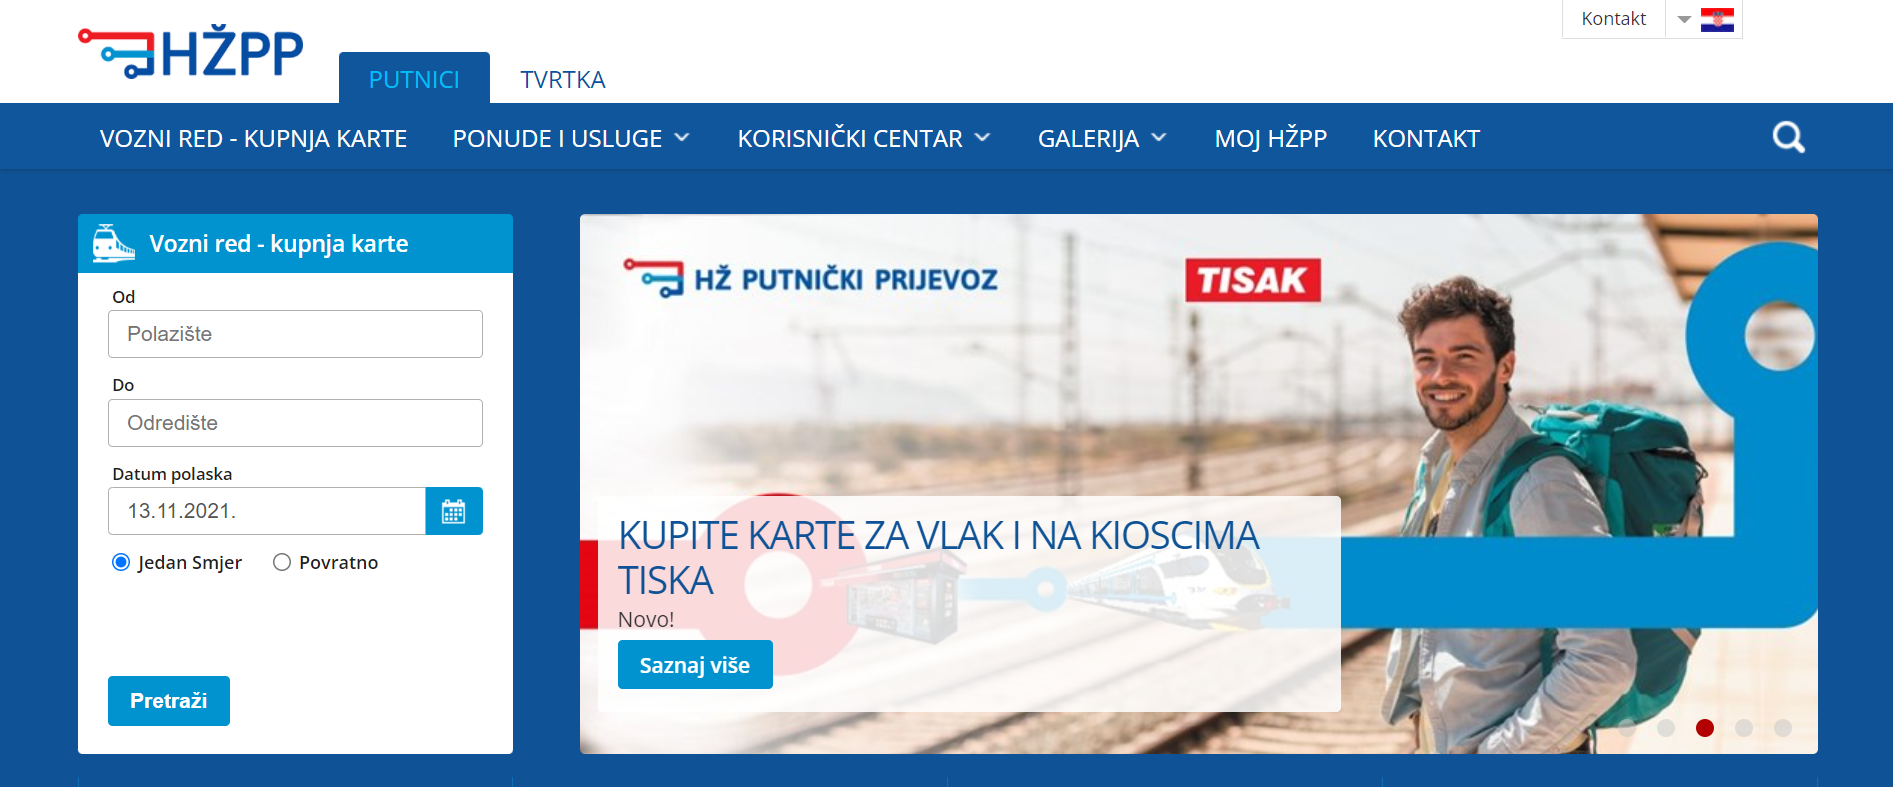
\includegraphics[width=1\linewidth]{"slike/hzpp.png"}
					\caption{Web stranica HŽPP-a}
					\label{fig:hzpp}
				\end{figure}
Također je tu i web aplikacija CityMapper koja sugerira korisniku mjesto sjedenja, no ne s obzirom na Gotcha sustav, nego s obzirom na korisnikove potrebe. Konkretnije, predlaže najbolje mjesto s obzirom na korisnikovo krajnje stajalište ili presjedanje. CityMapper posjeduje sve navedene funkcionalnosti kao i HŽPP web stranica.
 No, jako je malo web aplikacija koje sugeriraju korisniku koje mjesto bi bilo poželjno koristiti. 
 \begin{figure}[H]
					\centering
					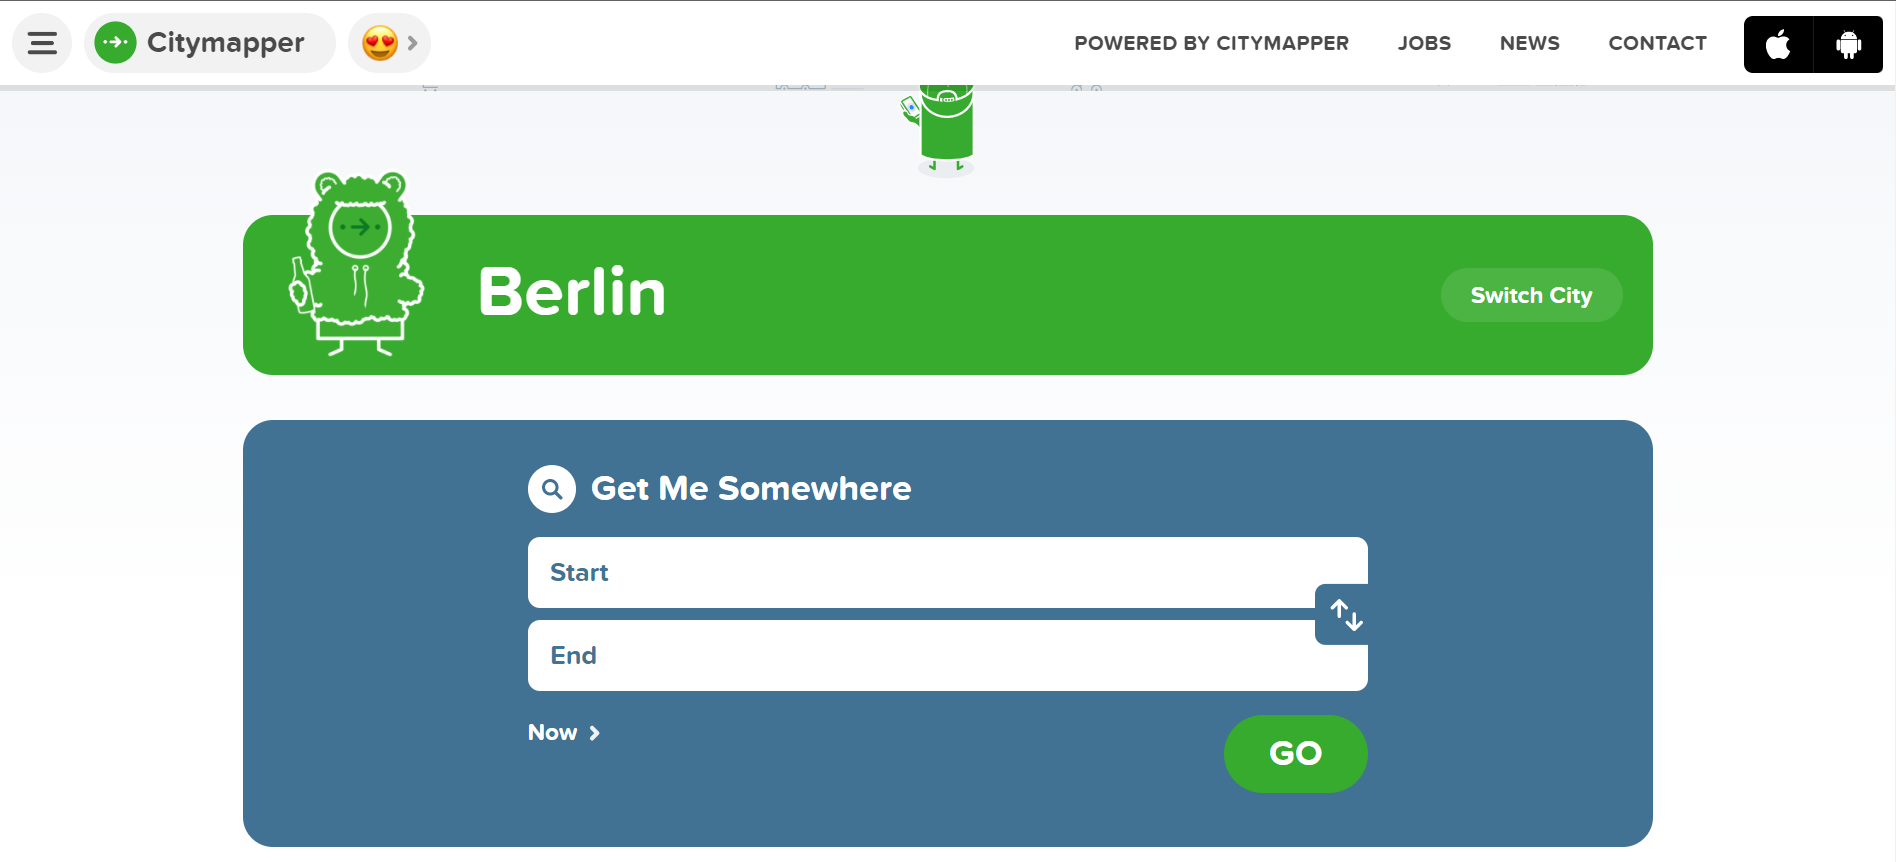
\includegraphics[width=1\linewidth]{"slike/cityMapper.png"}
					\caption{Web stranica cityMapper}
					\label{fig:cityMapper}
				\end{figure}


\textbf{Moguća nadogradnja:}\\
\begin{itemize}
    \item Web aplikaciju PassDirect bi se moglo unaprijediti dodavanjem novih funkcionalnosti poput zaključivanja o potrebi obnove infrastrukture na osnovu mjerenja senzora. Predviđanjem obnove, mogli bismo pravovremeno ukloniti određene vozne redove kako korisnik ne bi dobivao krivu informaciju pri ranoj kupovini karte ili ako dođe do otkazivanja linije, aplikacija bi trebala poslati e-mail korisniku.
    Uz to bi bila poželjna i funkcionalnost koja bi pri određivanju sjedala za korisnika, uz podatke mjerenja, uzimala u obzir i krajnje stajalište korisnika ili presjedanje i na taj način poticala korisnika još više da koristi upravo to određeno sjedalo, jer u tom slučaju, korist bi imao i korisnik i željeznički prijevoz. 
    \item Aplikaciju je moguće proširiti i na mobilnu platformu čime bi njena funkcionalnost bila fleksibilnija. Korisnik bi umjesto korištenja e-maila imao opciju čuvanja karte te dohvaćanja informacija o narednoj vožnji nakon kupovine na samoj mobilnoj aplikaciji. Također, bila bi olakšana komunikacija s korisnikom u slučaju promjena u redu vožnje (npr. promjena perona ili otkazivanja vožnje) putem notifikacija.
\end{itemize}



